%!TEX root = dissertacao.tex
% CAPA
\pagestyle{empty}
\begin{center}
\large  \textbf{UNIVERSIDADE PRESBITERIANA MACKENZIE}
\large  \textbf{PROGRAMA DE PÓS-GRADUAÇÃO EM}\\
\large  \textbf{ENGENHARIA ELÉTRICA E COMPUTAÇÃO}\\
\vskip 2.0cm
\textbf{\large Zorandir Soares Junior}\\
\vskip 4.0cm
\setlength{\baselineskip}{1.5\baselineskip}
\textbf{\large Diferença entre Templates de Autômatos Celulares Unidimensionais Binários}\\
\vskip 3.5cm
\end{center}
\vskip 7.3cm
\textbf{\normalsize Orientador: Prof. Dr. Pedro Paulo Balbi de Oliveira }\\
\vskip 1.0cm
\begin{center}
São Paulo\\
\the\year\\
\end{center}
\newpage

% CONTRACAPA
\pagestyle{empty}
\begin{center}
\large  \textbf{UNIVERSIDADE PRESBITERIANA MACKENZIE}
\large  \textbf{PROGRAMA DE PÓS-GRADUAÇÃO EM}\\
\large  \textbf{ENGENHARIA ELÉTRICA E COMPUTAÇÃO}\\
\vskip 2.0cm
\textbf{\large Zorandir Soares Junior}\\
\vskip 4.0cm
\setlength{\baselineskip}{1.5\baselineskip}
\textbf{\large Diferença entre Templates de Autômatos Celulares Unidimensionais Binários}\\
\vskip 3.5cm
\end{center}
\hfill{\vbox{\hsize=8.5cm\noindent\strut
Texto de dissertação apresentado ao \break
Programa de Pós-Graduação em Engenharia\break
Elétrica e Computação da Universidade\break
Presbiteriana Mackenzie como requisito das\break
exigências para obtenção do título de\break
Mestre em Engenharia Elétrica e Computação.\break}\\
\strut}
\vskip 3.0cm
\textbf{\normalsize Orientador: Prof. Dr. Pedro Paulo Balbi de Oliveira }\\
\vskip 1.0cm
\begin{center}
São Paulo\\
\the\year\\
\end{center}
\newpage

\pagestyle{empty}
\begin{center}
 $ \\ $
\vskip 12.5cm
\begin{figure}[h!]
\centering
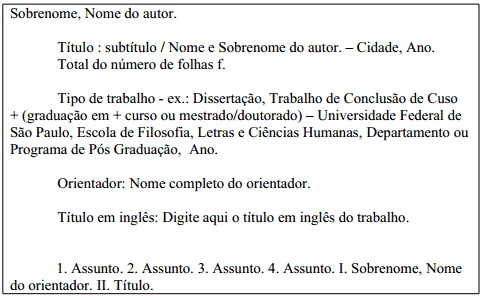
\includegraphics[width=0.75\textwidth]{ficha_catalografica.jpg}
\end{figure}
\vskip 1.0cm
\end{center}